%%%%%%%%%%%%%%%%%%%%%%%%%%%%%%%%%%%%%%%%%
% Lachaise Assignment
% LaTeX Template
% Version 1.0 (26/6/2018)
%
% This template originates from:
% http://www.LaTeXTemplates.com
%
% Authors:
% Marion Lachaise & François Févotte
% Vel (vel@LaTeXTemplates.com)
%
% License:
% CC BY-NC-SA 3.0 (http://creativecommons.org/licenses/by-nc-sa/3.0/)
% 
%%%%%%%%%%%%%%%%%%%%%%%%%%%%%%%%%%%%%%%%%

%----------------------------------------------------------------------------------------
%	PACKAGES AND OTHER DOCUMENT CONFIGURATIONS
%----------------------------------------------------------------------------------------

\documentclass{article}

%%%%%%%%%%%%%%%%%%%%%%%%%%%%%%%%%%%%%%%%%
% Lachaise Assignment
% Structure Specification File
% Version 1.0 (26/6/2018)
%
% This template originates from:
% http://www.LaTeXTemplates.com
%
% Authors:
% Marion Lachaise & François Févotte
% Vel (vel@LaTeXTemplates.com)
%
% License:
% CC BY-NC-SA 3.0 (http://creativecommons.org/licenses/by-nc-sa/3.0/)
% 
%%%%%%%%%%%%%%%%%%%%%%%%%%%%%%%%%%%%%%%%%

%----------------------------------------------------------------------------------------
%	PACKAGES AND OTHER DOCUMENT CONFIGURATIONS
%----------------------------------------------------------------------------------------

\usepackage{amsmath,amsfonts,stmaryrd,amssymb} % Math packages

\usepackage{enumerate} % Custom item numbers for enumerations

\usepackage[ruled]{algorithm2e} % Algorithms

\usepackage[framemethod=tikz]{mdframed} % Allows defining custom boxed/framed environments

\usepackage{listings} % File listings, with syntax highlighting
\lstset{
	basicstyle=\ttfamily, % Typeset listings in monospace font
}

%----------------------------------------------------------------------------------------
%	DOCUMENT MARGINS
%----------------------------------------------------------------------------------------

\usepackage{geometry} % Required for adjusting page dimensions and margins

\geometry{
	paper=a4paper, % Paper size, change to letterpaper for US letter size
	top=2.5cm, % Top margin
	bottom=3cm, % Bottom margin
	left=2.5cm, % Left margin
	right=2.5cm, % Right margin
	headheight=14pt, % Header height
	footskip=1.5cm, % Space from the bottom margin to the baseline of the footer
	headsep=1.2cm, % Space from the top margin to the baseline of the header
	%showframe, % Uncomment to show how the type block is set on the page
}

%----------------------------------------------------------------------------------------
%	FONTS
%----------------------------------------------------------------------------------------

\usepackage[utf8]{inputenc} % Required for inputting international characters
\usepackage[T1]{fontenc} % Output font encoding for international characters

\usepackage{XCharter} % Use the XCharter fonts

%----------------------------------------------------------------------------------------
%	COMMAND LINE ENVIRONMENT
%----------------------------------------------------------------------------------------

% Usage:
% \begin{commandline}
%	\begin{verbatim}
%		$ ls
%		
%		Applications	Desktop	...
%	\end{verbatim}
% \end{commandline}

\mdfdefinestyle{commandline}{
	leftmargin=10pt,
	rightmargin=10pt,
	innerleftmargin=15pt,
	middlelinecolor=black!50!white,
	middlelinewidth=2pt,
	frametitlerule=false,
	backgroundcolor=black!5!white,
	frametitle={Command Line},
	frametitlefont={\normalfont\sffamily\color{white}\hspace{-1em}},
	frametitlebackgroundcolor=black!50!white,
	nobreak,
}

% Define a custom environment for command-line snapshots
\newenvironment{commandline}{
	\medskip
	\begin{mdframed}[style=commandline]
}{
	\end{mdframed}
	\medskip
}

%----------------------------------------------------------------------------------------
%	FILE CONTENTS ENVIRONMENT
%----------------------------------------------------------------------------------------

% Usage:
% \begin{file}[optional filename, defaults to "File"]
%	File contents, for example, with a listings environment
% \end{file}

\mdfdefinestyle{file}{
	innertopmargin=1.6\baselineskip,
	innerbottommargin=0.8\baselineskip,
	topline=false, bottomline=false,
	leftline=false, rightline=false,
	leftmargin=2cm,
	rightmargin=2cm,
	singleextra={%
		\draw[fill=black!10!white](P)++(0,-1.2em)rectangle(P-|O);
		\node[anchor=north west]
		at(P-|O){\ttfamily\mdfilename};
		%
		\def\l{3em}
		\draw(O-|P)++(-\l,0)--++(\l,\l)--(P)--(P-|O)--(O)--cycle;
		\draw(O-|P)++(-\l,0)--++(0,\l)--++(\l,0);
	},
	nobreak,
}

% Define a custom environment for file contents
\newenvironment{file}[1][File]{ % Set the default filename to "File"
	\medskip
	\newcommand{\mdfilename}{#1}
	\begin{mdframed}[style=file]
}{
	\end{mdframed}
	\medskip
}

%----------------------------------------------------------------------------------------
%	NUMBERED QUESTIONS ENVIRONMENT
%----------------------------------------------------------------------------------------

% Usage:
% \begin{question}[optional title]
%	Question contents
% \end{question}

\mdfdefinestyle{question}{
	innertopmargin=1.2\baselineskip,
	innerbottommargin=0.8\baselineskip,
	roundcorner=5pt,
	nobreak,
	singleextra={%
		\draw(P-|O)node[xshift=1em,anchor=west,fill=white,draw,rounded corners=5pt]{%
		Question \theQuestion\questionTitle};
	},
}

\newcounter{Question} % Stores the current question number that gets iterated with each new question

% Define a custom environment for numbered questions
\newenvironment{question}[1][\unskip]{
	\bigskip
	\stepcounter{Question}
	\newcommand{\questionTitle}{~#1}
	\begin{mdframed}[style=question]
}{
	\end{mdframed}
	\medskip
}

%----------------------------------------------------------------------------------------
%	WARNING TEXT ENVIRONMENT
%----------------------------------------------------------------------------------------

% Usage:
% \begin{warn}[optional title, defaults to "Warning:"]
%	Contents
% \end{warn}

\mdfdefinestyle{warning}{
	topline=false, bottomline=false,
	leftline=false, rightline=false,
	nobreak,
	singleextra={%
		\draw(P-|O)++(-0.5em,0)node(tmp1){};
		\draw(P-|O)++(0.5em,0)node(tmp2){};
		\fill[black,rotate around={45:(P-|O)}](tmp1)rectangle(tmp2);
		\node at(P-|O){\color{white}\scriptsize\bf !};
		\draw[very thick](P-|O)++(0,-1em)--(O);%--(O-|P);
	}
}

% Define a custom environment for warning text
\newenvironment{warn}[1][Warning:]{ % Set the default warning to "Warning:"
	\medskip
	\begin{mdframed}[style=warning]
		\noindent{\textbf{#1}}
}{
	\end{mdframed}
}

%----------------------------------------------------------------------------------------
%	INFORMATION ENVIRONMENT
%----------------------------------------------------------------------------------------

% Usage:
% \begin{info}[optional title, defaults to "Info:"]
% 	contents
% 	\end{info}

\mdfdefinestyle{info}{%
	topline=false, bottomline=false,
	leftline=false, rightline=false,
	nobreak,
	singleextra={%
		\fill[black](P-|O)circle[radius=0.4em];
		\node at(P-|O){\color{white}\scriptsize\bf i};
		\draw[very thick](P-|O)++(0,-0.8em)--(O);%--(O-|P);
	}
}

% Define a custom environment for information
\newenvironment{info}[1][Info:]{ % Set the default title to "Info:"
	\medskip
	\begin{mdframed}[style=info]
		\noindent{\textbf{#1}}
}{
	\end{mdframed}
}
 % Include the file specifying the document structure and custom commands

%----------------------------------------------------------------------------------------
%	ASSIGNMENT INFORMATION
%----------------------------------------------------------------------------------------

\title{Introduction to Artificial Intelligence: Assignment \#1\\Fast Trajectory Replanning} % Title of the assignment

\author{Yuyang Chen. -- yc791\\ Simiao fan -- sf578\\ Zhaohan Yan -- zy134} % Author name and email address

\date{Rutgers University --- \today} % University, school and/or department name(s) and a date

%----------------------------------------------------------------------------------------

\begin{document}

\maketitle % Print the title

%----------------------------------------------------------------------------------------
%	INTRODUCTION
%----------------------------------------------------------------------------------------

\section*{Introduction} % Unnumbered section

\begin{info} % Information block
	This document is Homework 1 for 198:440 Introduction to Artificial Intelligence at Rutgers University Spring 2019.
\end{info}

%----------------------------------------------------------------------------------------
%	Part 1 - Understanding the methods
%----------------------------------------------------------------------------------------

\section{Part 1 - Understanding the methods} % Numbered section

Read the chapter in your textbook on uninformed and informed
(heuristic) search and then read the project description again. Make sure that you understand A* and the concepts of
admissible and consistent h-values.

%------------------------------------------------

\subsection{}

% Numbered question, with subquestions in an enumerate environment
\begin{question}
	Explain in your report why the first move of the agent for the example search problem from Figure 8 is to the east rather
than the north given that the agent does not know initially which cells are blocked.

\end{question}

Answer: \newline
\par When the agent begins in the maze program, it does not initially know which cells are blocked. It has to survey its surroundings as it takes each proceeding step. In Figure 8, the agent takes a step to the east rather than north because A* would calculate that it would take a shorter distance to the goal to go east, rather than first north and then east. Our agent can only see which cells are blocked at each subsequent step, so at its initial position, it cannot see that the path directly east is blocked both to the right and from above. Only once it moves east will it realize that it is not the correct path, and then move back to go north.
	
%------------------------------------------------

\subsection{}

% Numbered question, with subquestions in an enumerate environment
\begin{question}
	This project argues that the agent is guaranteed to reach the target if it is not separated from it by blocked cells. Give a
convincing argument that the agent in finite gridworlds indeed either reaches the target or discovers that this is impossible
in finite time. Prove that the number of moves of the agent until it reaches the target or discovers that this is impossible is
bounded from above by the number of unblocked cells squared.

\end{question}

Answer: \newline
\par In this gridworld, the agent is guaranteed to reach the target of the maze (goal) or discover it is impossible to as A* search leads our agent through every possible cell in the grid to the goal. If the agent detect that the goal state is blocked on all sides by obstacles such as the grid edge or blocked cells, in the next A* search, the open list would be empty before the the algorithm pushing the goal stage node into the open list, and therefore we know we can’t reach to the goal stage. Otherwise, the agent will keep moving along each cell until it reaches goal.

Use induction to prove: "The number of moves of the agent until it reaches the target or discovers that this is impossible is bounded from above by the number of unblocked cells squared. Let n be the total number of cells, let m be the number of unblocked cells, and let k be the
total number of moves the agent took

Base case: n = 2, when there is only start state and goal state. If the goal state is blocked,
then the total move would be k = 0, m = 1.

$$k < m^2  --- check$$

If the goal state is unblocked, then m = 2, k = 1, because we directly move from start to goal with a single step. 

$$k < m^2 --- check$$

Inductive step: For n > 2, Suppose 

$$k < m'^2$$
 
is true for all  m' belong [1, m),need to prove $$k < m^2$$ is also true. We know that for each unblocked cell, the agent would at most visit it twice (the first time follow the path to the goal, and later come back with the updated blocked information). Therefore, $k <= 2m.$ 

$$(\frac{2m}{m^2}) = (\frac{2}{m})$$, 

since $m > m' >= 1,$ therefore $m >= 2,$ and further 

$$(\frac{2}{m}) <= 1$$. 

Thus k'/2m <= 1. Therefore $k < m^2$ hold true.
Based on the base step and inductive step, we know $k < m^2$ for all m >= 1.



%----------------------------------------------------------------------------------------
%	Part 2 - The Effect of Ties
%----------------------------------------------------------------------------------------

\section{Part 2 - The Effect of Ties}

Repeated Forward A* needs to break ties to decide which cell to expand next if
several cells have the same smallest f-value. It can either break ties in favor of cells with smaller g-values or in favor of
cells with larger g-values. Implement and compare both versions of Repeated Forward A* with respect to their runtime or,
equivalently, number of expanded cells.

%------------------------------------------------

% Numbered question, with subquestions in an enumerate environment
\begin{question}
	Explain your observations in detail, that is, explain what you observed and give a
reason for the observation.

\end{question}

Answer: \newline
\par First, we use the breaking tie as 100*100 as larger value, and then we set it as 50*50 as smaller value

Repeated Forward A*

\textbf{Choosing smaller g-value}
Average run time: 0.553608422583722

\textbf{Choosing larger g-value}
Average run time: 0.594 s


We observed that tie-breaking by the larger g-value proved to be almost ten times faster than the other method. From the A* algorithm, f(s) = g(s) + h(s). In terms of the tie-breaking, we can conclude that having a bigger g-value also means having a smaller h-value. In our case, the g-value represents the cost of the path the agent has finished while the h-value is a prediction of the best case in the future which can potentially increase a lot. In other words, having a larger h-value gives the agent more risks of increasing its overall cost in the future. With the same f-values, the one with the larger g-value will more likely to finish its path with less cost to be added to its original prediction. It is also why the method of choosing the larger g-value is faster than the method of choosing the smaller g-value.

% File contents
\begin{file}[hello.py]
\begin{lstlisting}[language=Python]
#! /usr/bin/python

import sys
sys.stdout.write("Hello World!\n")
\end{lstlisting}
\end{file}

Fusce eleifend porttitor arcu, id accumsan elit pharetra eget. Mauris luctus velit sit amet est sodales rhoncus. Donec cursus suscipit justo, sed tristique ipsum fermentum nec. Ut tortor ex, ullamcorper varius congue in, efficitur a tellus. Vivamus ut rutrum nisi. Phasellus sit amet enim efficitur, aliquam nulla id, lacinia mauris. Quisque viverra libero ac magna maximus efficitur. Interdum et malesuada fames ac ante ipsum primis in faucibus. Vestibulum mollis eros in tellus fermentum, vitae tristique justo finibus. Sed quis vehicula nibh. Etiam nulla justo, pellentesque id sapien at, semper aliquam arcu. Integer at commodo arcu. Quisque dapibus ut lacus eget vulputate.

% Command-line "screenshot"
\begin{commandline}
	\begin{verbatim}
		$ chmod +x hello.py
		$ ./hello.py

		Hello World!
	\end{verbatim}
\end{commandline}

Vestibulum sodales orci a nisi interdum tristique. In dictum vehicula dui, eget bibendum purus elementum eu. Pellentesque lobortis mattis mauris, non feugiat dolor vulputate a. Cras porttitor dapibus lacus at pulvinar. Praesent eu nunc et libero porttitor malesuada tempus quis massa. Aenean cursus ipsum a velit ultricies sagittis. Sed non leo ullamcorper, suscipit massa ut, pulvinar erat. Aliquam erat volutpat. Nulla non lacus vitae mi placerat tincidunt et ac diam. Aliquam tincidunt augue sem, ut vestibulum est volutpat eget. Suspendisse potenti. Integer condimentum, risus nec maximus elementum, lacus purus porta arcu, at ultrices diam nisl eget urna. Curabitur sollicitudin diam quis sollicitudin varius. Ut porta erat ornare laoreet euismod. In tincidunt purus dui, nec egestas dui convallis non. In vestibulum ipsum in dictum scelerisque.

%----------------------------------------------------------------------------------------
%	Part 3 - Forward vs. Backward
%----------------------------------------------------------------------------------------

\section{Part 3 - Forward vs. Backward}

Implement and compare Repeated Forward A* and Repeated Backward A*
with respect to their runtime or, equivalently, number of expanded cells. Explain your observations in detail, that is, explain
what you observed and give a reason for the observation. Both versions of Repeated A* should break ties among cells with
the same f-value in favor of cells with larger g-values and remaining ties in an identical way, for example randomly
\newline

%------------------------------------------------

Answer: \newline
\textbf{Repeated Forward A*:}
{\obeylines\obeyspaces
\texttt{
\input{RepeatedForwardOutput.txt}
}}
\textbf{Repeated Forward A*: Average run time = 0.3089696089426676}
\newline
\textbf{Repeated Forward A*: Average expanded node = 3959.15555556}
\newline
\newline
\textbf{Repeated Backward A*:}
{\obeylines\obeyspaces
\texttt{
\input{RepeatedBackwardOutput.txt}
}}
\textbf{Repeated Backward A*: Average run time = 0.3506512123605479}
\newline
\textbf{Repeated Backward A*: Average expanded node = 176390.76087}
\par Obersvation : After comparing the run time and the number of expanded node of Repeated Forward and Backward, we can easily find that Repeated Forward A* ran faster than Backward A. But in this situation, the origin node and destination node are not the same.
\newline
By setting another python file to test, we set the origin node is same as the destination node. We use it to compare it again:
\newline
\newline
\newline
Repeated Forward:
\newline
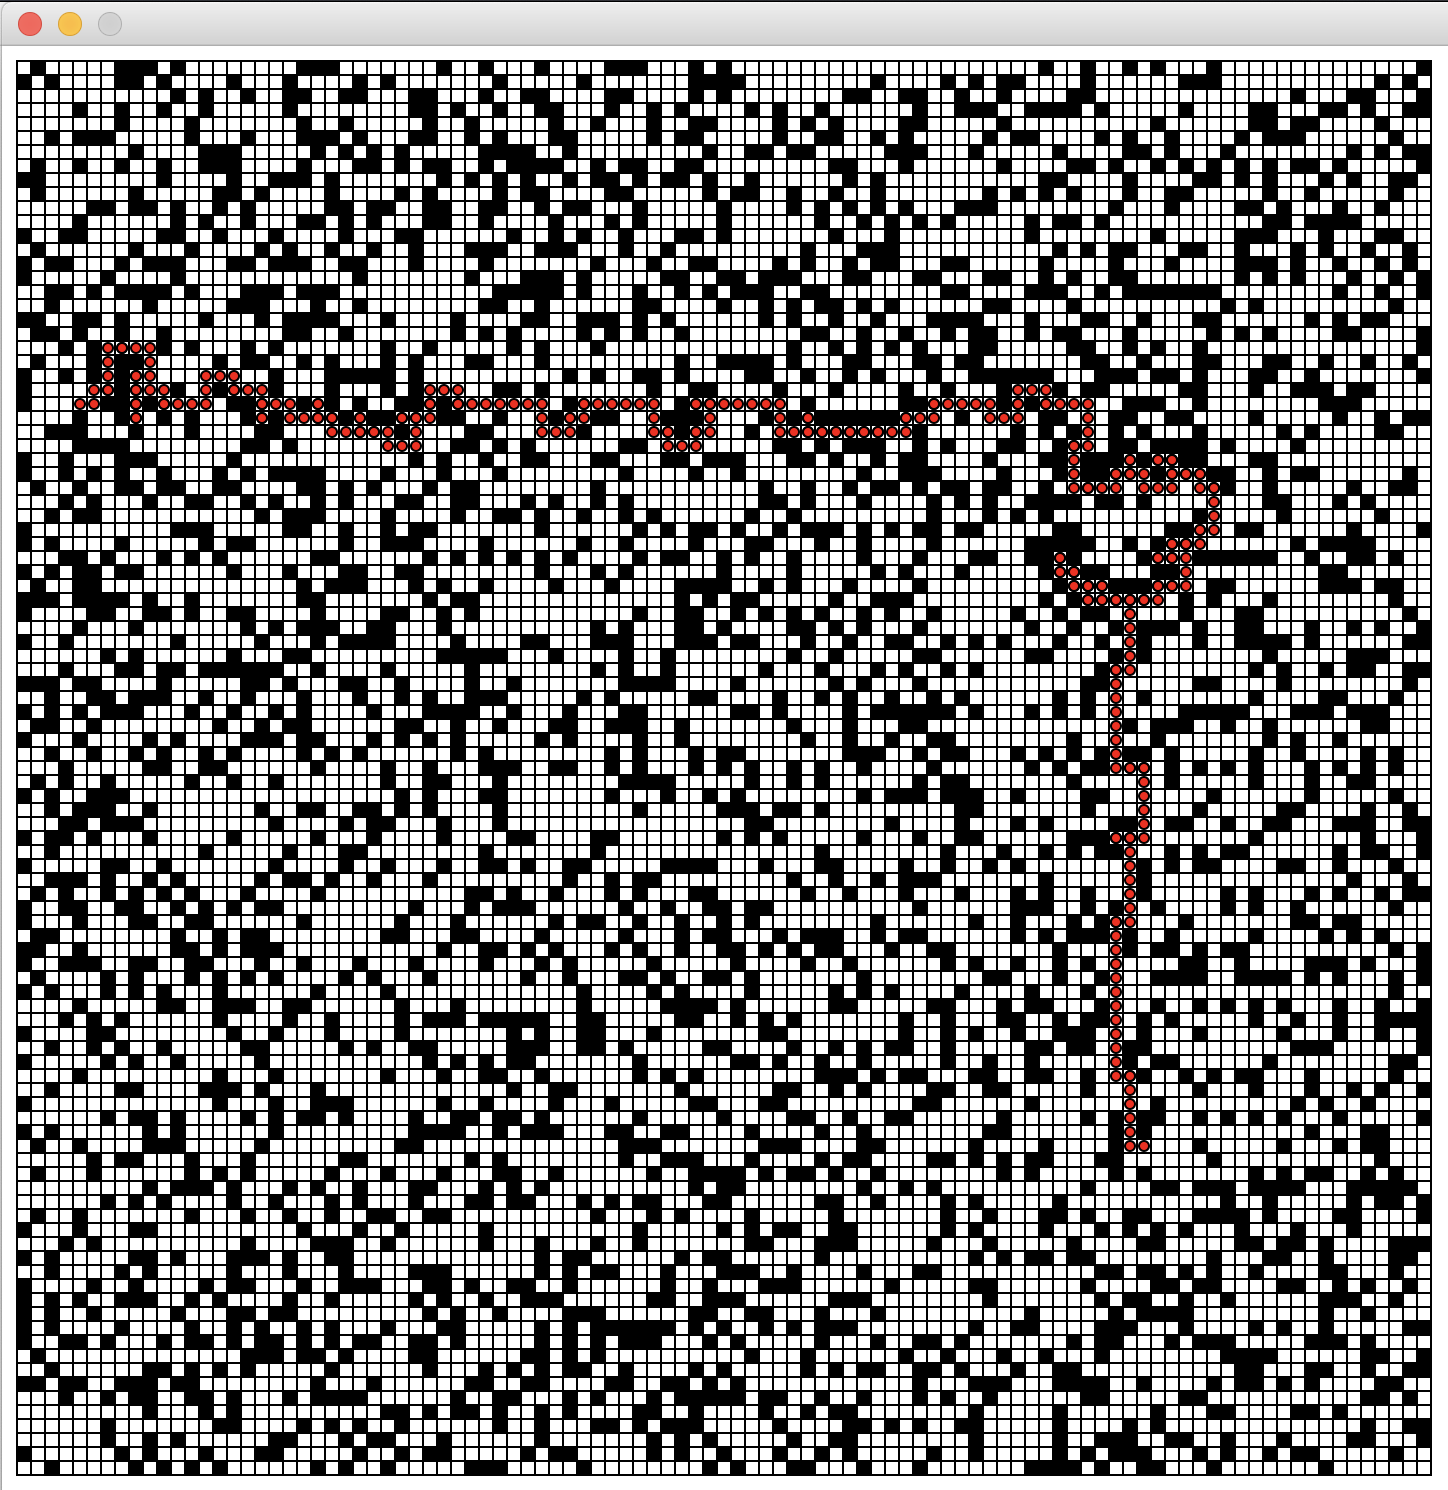
\includegraphics[scale = 0.70]{forward.PNG}
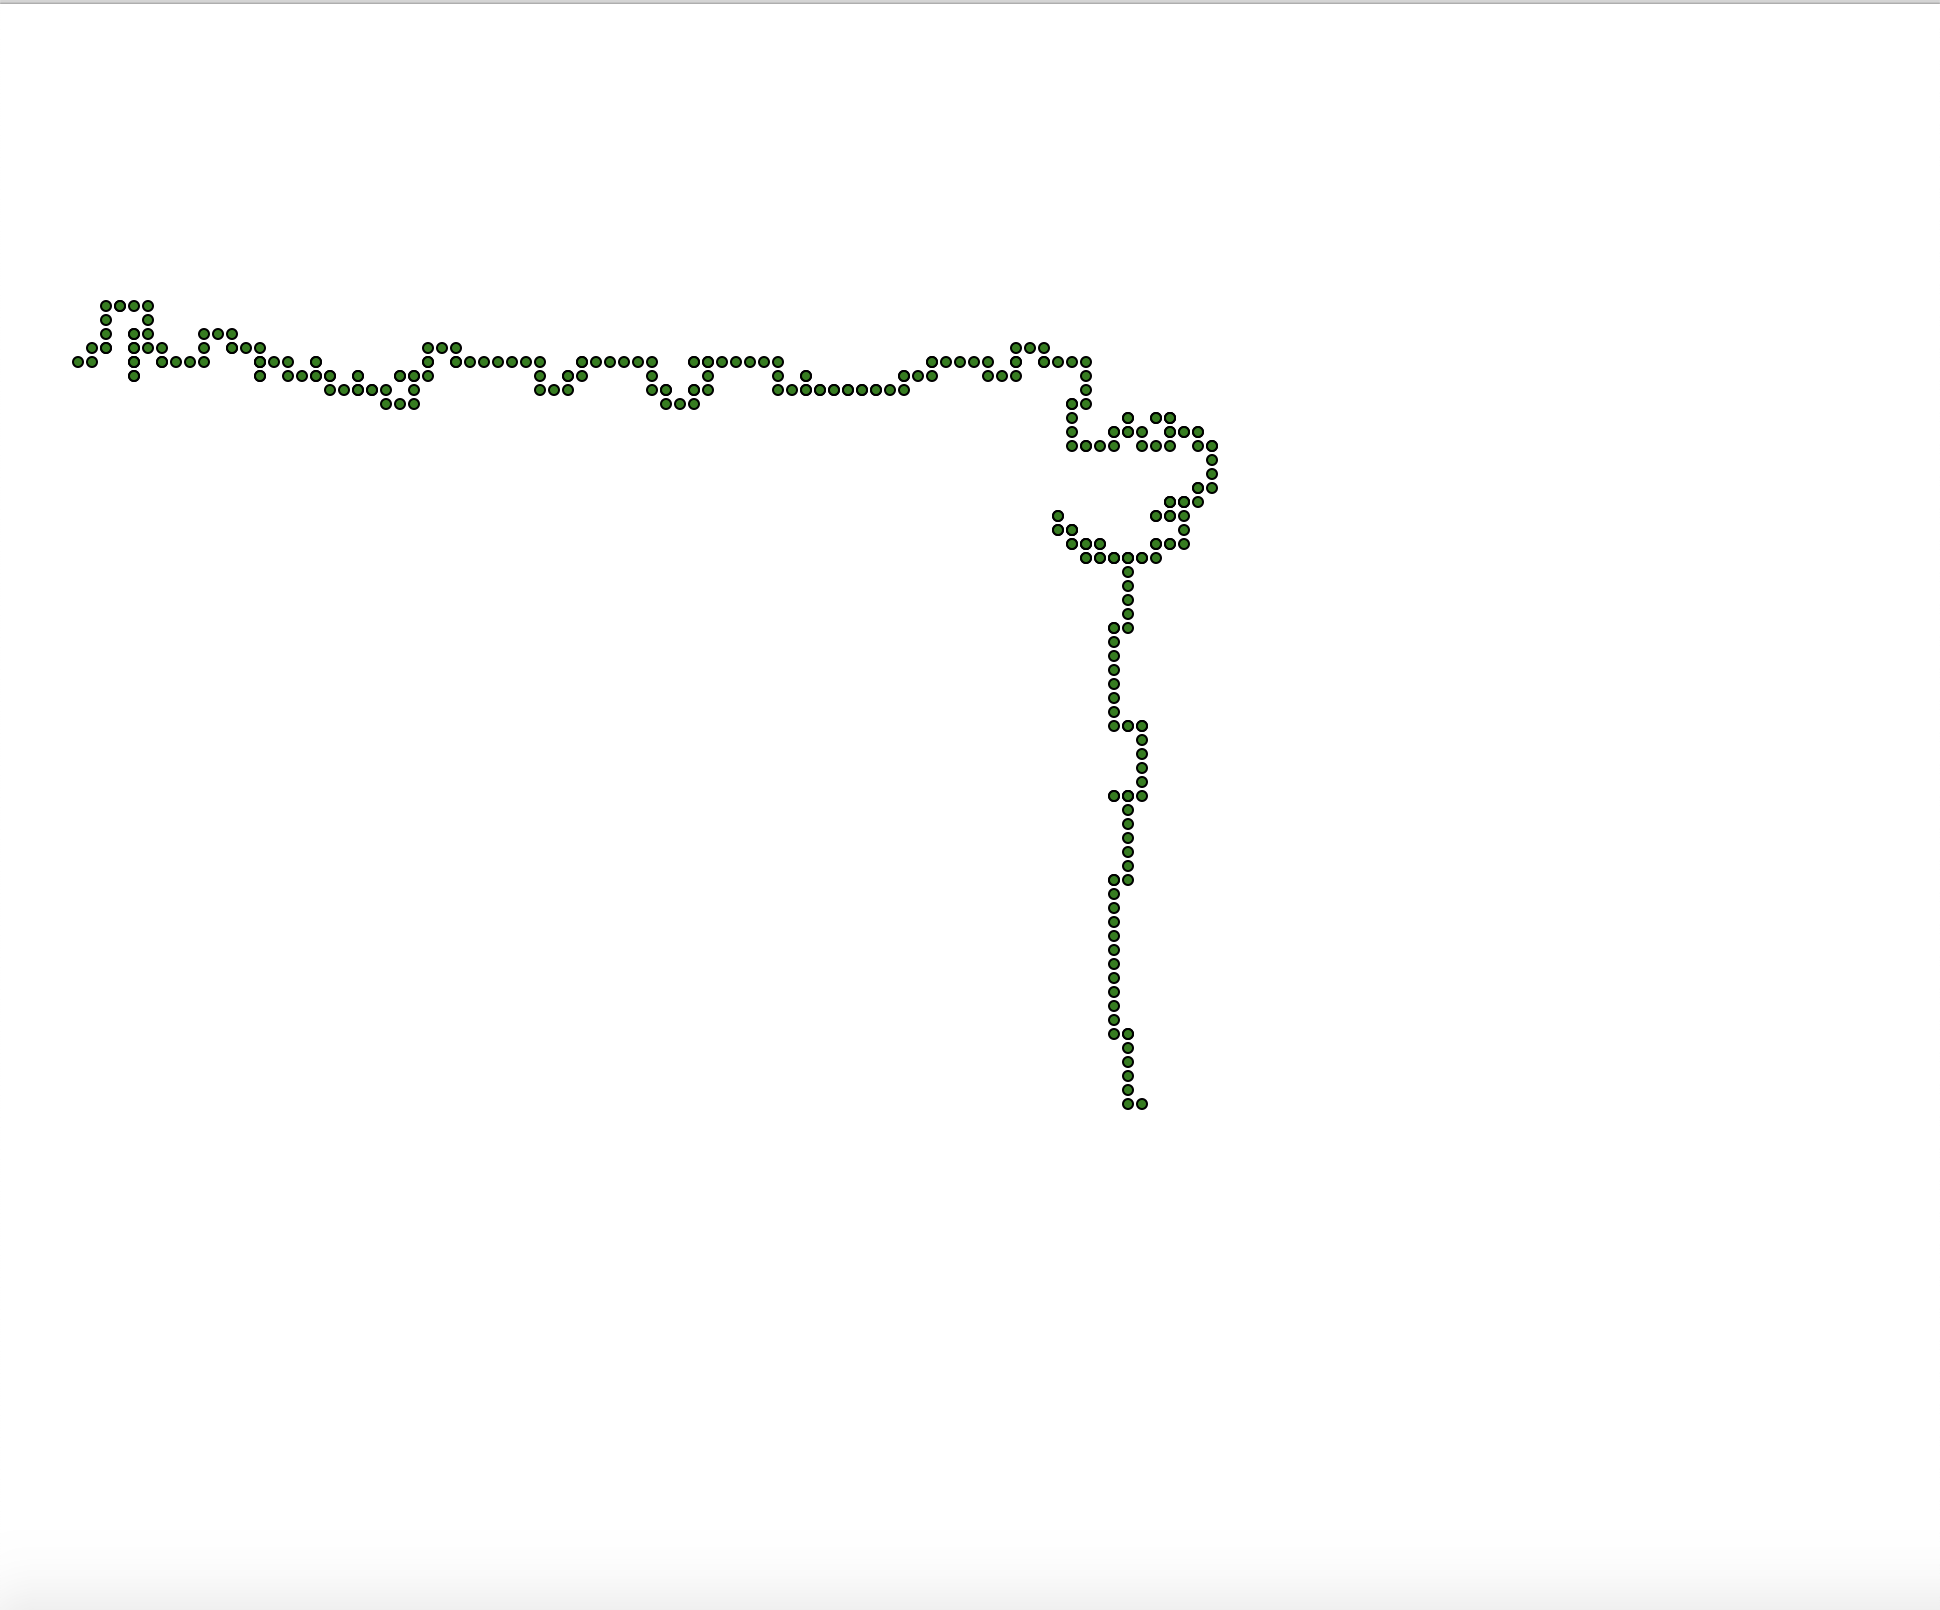
\includegraphics[scale = 0.70]{forward2.PNG}
\newline
Repeated Backward:
\newline
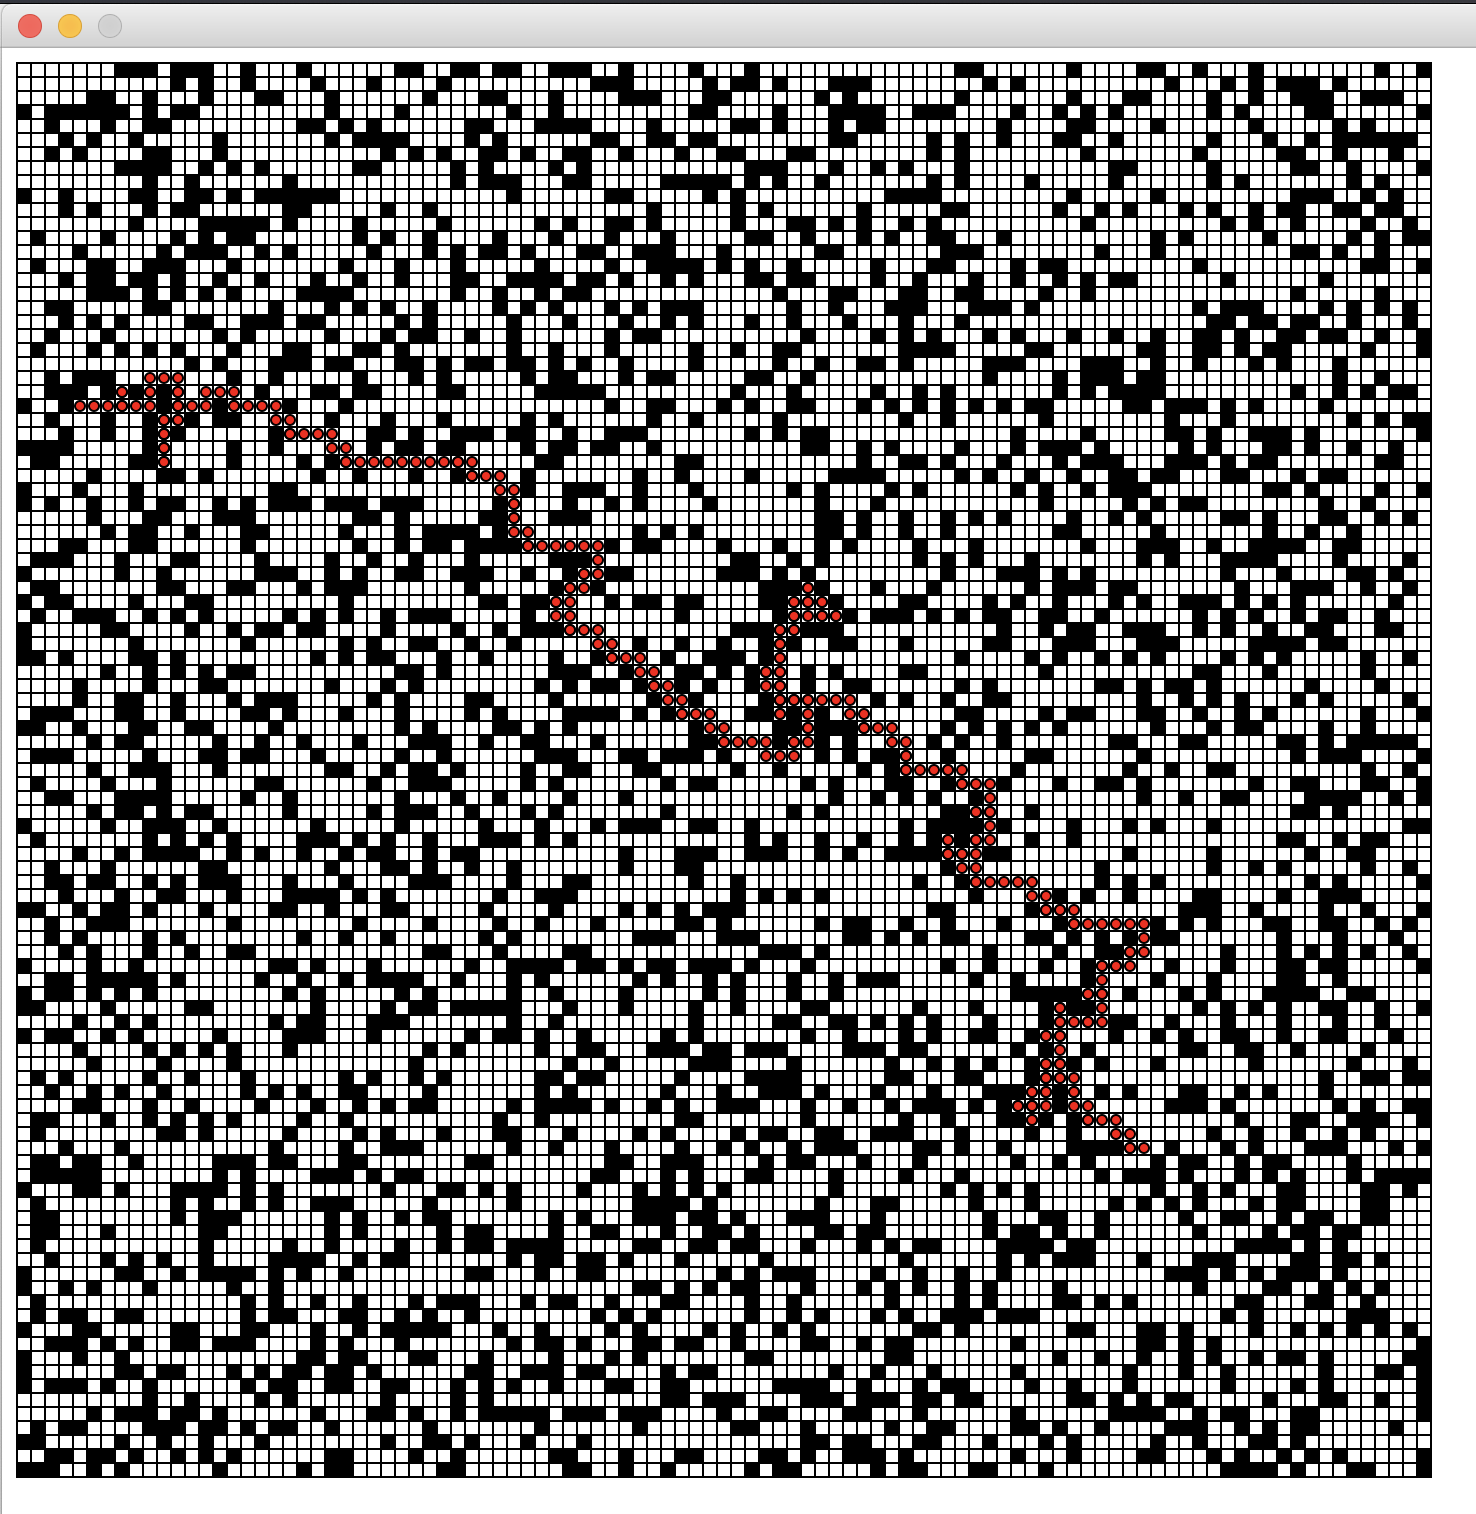
\includegraphics[scale = 0.70]{backward.PNG}
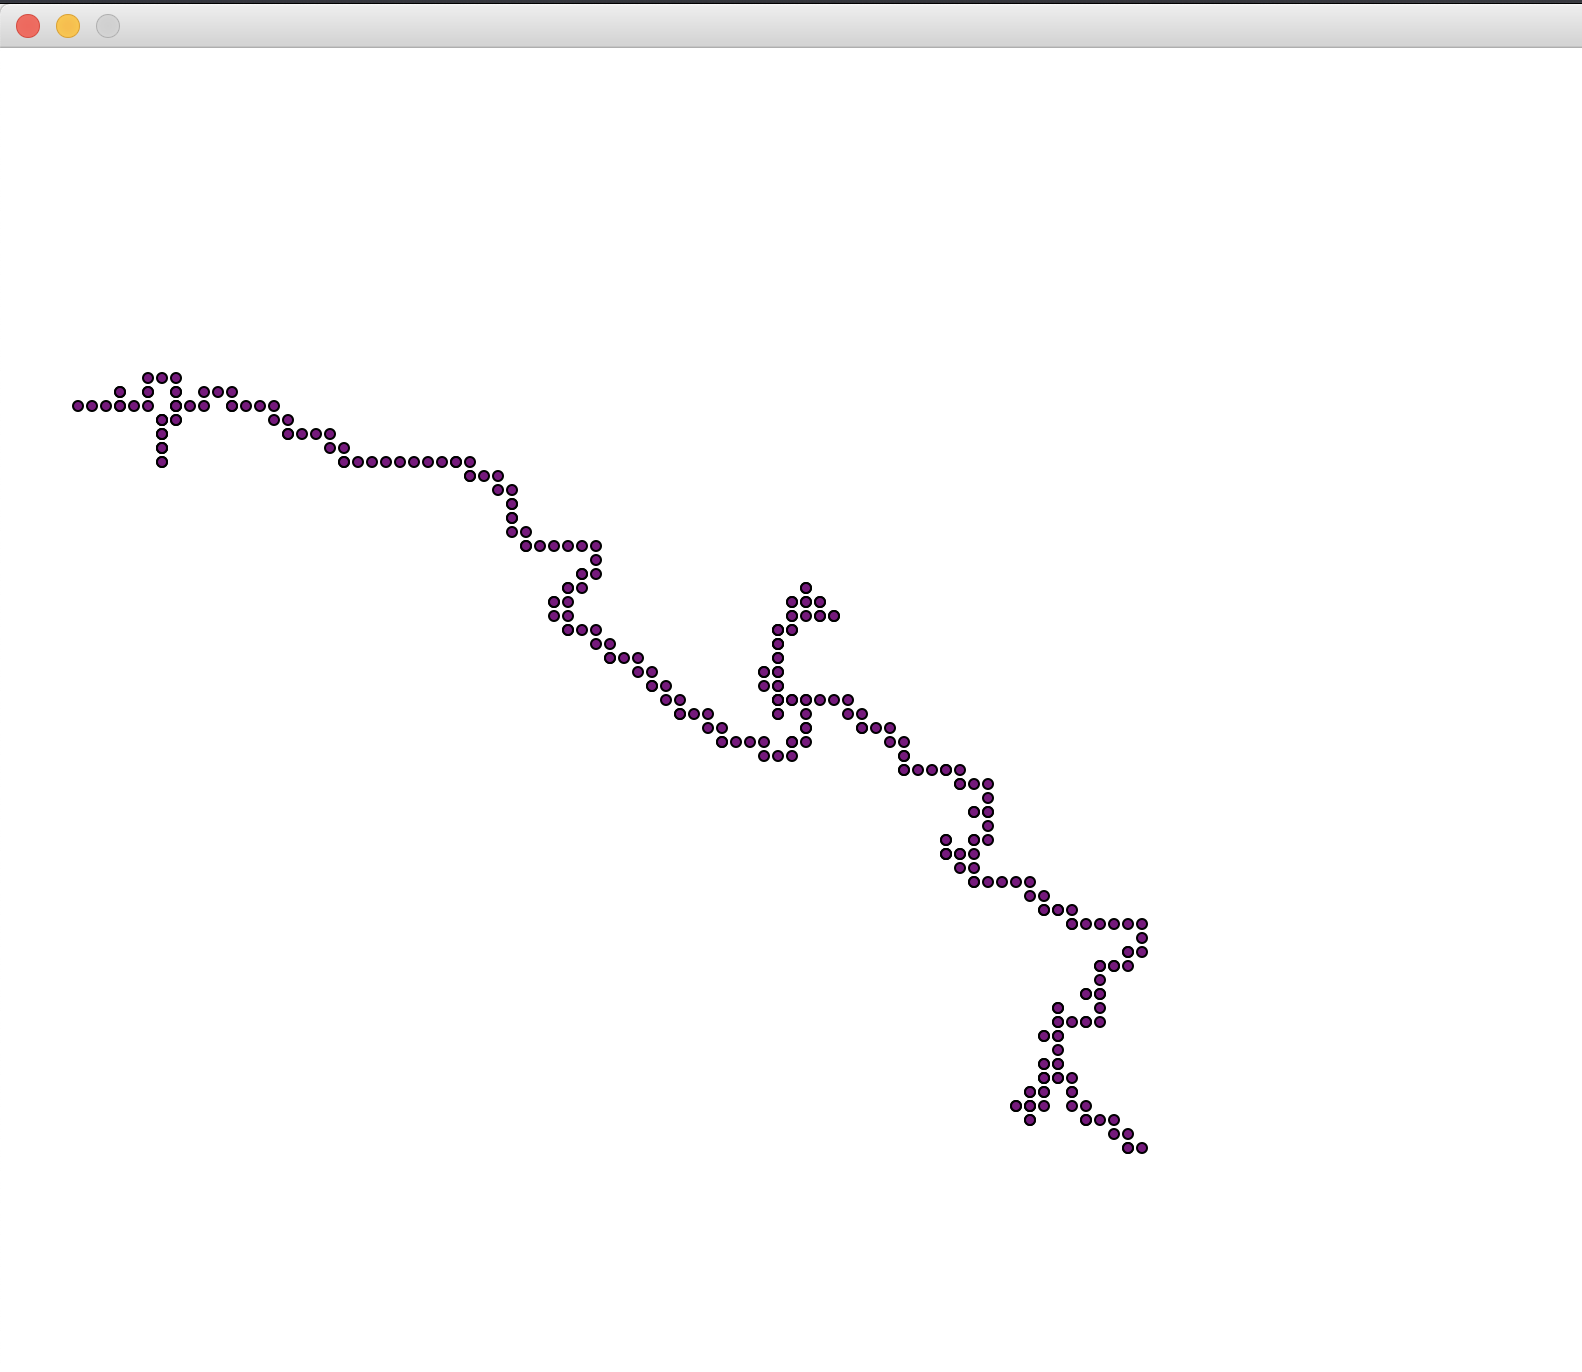
\includegraphics[scale = 0.70]{backward2.PNG}
\newline
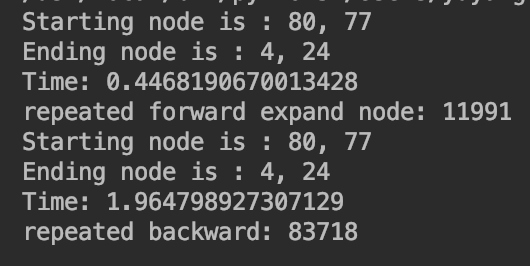
\includegraphics[scale = 0.70]{Output.PNG}
\newline
\par By comparing these two condition, we can easily say that the running time of Repeated Forward A* is obviously faster than the Repeated Backward A*.
\newline
\newline
Explanation: Here, we know the repeated backward need to expand more cells, (83718 >> 11991). During one iteration of the A* search, we start the search from a place very close to the already detected vertical obstacle, then the A* search would find the break point vertically step by step, in which case each step starts over from the beginning to the next vertical point of the obstacle. For the 

%----------------------------------------------------------------------------------------
%	Part 4 - Heuristics in the Adaptive A*
%----------------------------------------------------------------------------------------

\section{Part 4 - Heuristics in the Adaptive A*}

The project argues that “the Manhattan distances are consistent in
gridworlds in which the agent can move only in the four main compass directions.” Prove that this is indeed the case.

Furthermore, it is argued that “The h-values hnew(s) ... are not only admissible but also consistent.” Prove that Adaptive A*
leaves initially consistent h-values consistent even if action costs can increase.
\newline

%------------------------------------------------

Answer: \newline
The heuristic function h is said to be consistent if 
$$ \forall(n, a, n'): h(n) \leq c(n, a, n') + h(n'),$$
where c(n, a, n') is the step cost for going from n to n' using action a.
\par In this case, the step cost for each move is 1, therefore, $$c(n, a, n') + h(n') = h(n') + 1$$ , and h(n) is either h(n') + 1 or h(n') - 1, whenever the agent makes the next move. \par In the case of h(n) = h(n') + 1, h(n) = c(n, a, n') + h(n'). \par In the case of h(n) = h(n') - 1, h(n) < c(n, a, n') + h(n').
\par Thus, the statement "the Manhattan distances are consistent in grid-worlds in which the agent can move only in the four main compass directions" is true.



$$$$\par The second part asks us to prove that Adaptive A* leaves initially consistent h-values consistent even if action costs can increase. The heuristic function h is said to be consistent if 
$$ \forall(n, a, n'): h(n) \leq c(n, a, n') + h(n'),$$ where c(n, a, n') is the step cost for going from n to n' using action a.
\par For each Adaptive process, let the step cost for each move to be denoted by the variable A where A is an integer greater than 0, thus, $$c(n, a, n') + h(n') = h(n') + A$$ . 
\par As is known, for Adaptive A* search, $h_{new} = g(s_{goal}) - g(s)$, and we need to prove:
$$h_{new}(s) \leq h_{new}(s') + A,$$ 
\par which is equal to:
$$g(s_{goal}) - g(s) \leq g(s_{goa})) - g(s') + A$$
$$ => g(s') \leq (s) + A,$$ 
\par which is true.
\par Thus, the statement "Adaptive A* leaves initially consistent h-values consistent even if action costs can increase" is true.

%----------------------------------------------------------------------------------------
%	Part 5 - Heuristics in the Adaptive A*
%----------------------------------------------------------------------------------------

\section{Part 5 - Heuristics in the Adaptive A*}

Implement and compare Repeated Forward A* and Adaptive A*
with respect to their runtime. Explain your observations in detail, that is, explain what you observed and give a reason for
the observation. Both search algorithms should break ties among cells with the same f-value in favor of cells with larger
g-values and remaining ties in an identical way, for example randomly.
\newline

%------------------------------------------------

Answer: \newline

\par 

%----------------------------------------------------------------------------------------
%	Part 6 - Memory Issues
%----------------------------------------------------------------------------------------

\section{Part 6 - Memory Issues}

You performed all experiments in gridworlds of size 101 × 101 but some real-time
computer games use maps whose number of cells is up to two orders of magnitude larger than that. It is then especially
important to limit the amount of information that is stored per cell. For example, the tree-pointers can be implemented with
only two bits per cell. Suggest additional ways to reduce the memory consumption of your implementations further. Then,
calculate the amount of memory that they need to operate on gridworlds of size 1001 × 1001 and the largest gridworld that
they can operate on within a memory limit of 4 MBytes.
\newline

%------------------------------------------------

Answer: \newline
\par In regards to memory consumption, there are a couple of strategies that can be taken in order to reduce it. One method would be to use different variable types in order to save on some space. One simple example, for a variable that indicates whether a cell is blocked or not, this should be a simple boolean value rather than a numerical value. Another would be to limit the number of variables associated with our node class and store less information in general in each node. One of the most important ways is to examine our data structures and see if we may have implemented any other types to save on memory consumption. Another way is to avoid generating the entire map on the agent’s side, and only update the nodes that the agent observes. By storing the fog of war, we are unnecessarily using space when the agent can simply create the map as it walks along the grid-world. Our implementation does this but we can see other versions of this project unnecessarily doing this.
Furthermore, we can even put the information of all fields inside of one field. For example, our old class cell is written as:

\begin{lstlisting}
class Cell:
    def __init__(self, xPos, yPos, if_blocked, ifVisited=False):
        self.x = xPos
        self.y = yPos
        self.ifBlocked = if_blocked
        self.visited = ifVisited

\end{lstlisting}


For the sake of saving memory, our new class cell can be written as the following with get's methods:
\begin{lstlisting}
class Cell:
	def __init__(self, xPos, yPos, if_blocked, ifVisited):
    	# xPos is the 4-digit x-coordinate, yPos is the 4-digit y-coordinate
        # if_blocked and ifVisited either 1 or 0 in order to indicate a boolean variable
        self.xxxxyyyybv = xPos*1000000+yPos*100+if_blocked*10+ifVisited

	def getx(self):
        temp = self.xxxxyyyybv
        return int(temp / 1000000)

	def gety(self):
        temp = self.xxxxyyyybv - getx(self) * 1000000
        return int(temp / 100)

	def getIfBlokced(self):
        temp = self.xxxxyyyybv - getx(self) * 1000000 - gety(self) * 100
        return int(temp /10)

	def getIfVisited(self):
        temp = self.xxxxyyyybv
        return temp % 2
\end{lstlisting}


\par In this way, each object we create will just be an int type and an int type has a size of 4 bytes and we can do something similar to the class node. Let's take 4MB as 4e6 bytes, then the maximum number of grids we can have will be 4e6/4/2 = 500000. $\sqrt{500000}=707$, which means we will support a 707x707 grid-world for the worst case. For a 1001x1001 grid-world, it will take 1001*1001*4*2 = 8016008 bytes of memory which is roughly 8 MB of memory.
%----------------------------------------------------------------------------------------

\end{document}
